\documentclass[a4paper,12pt]{article}

\usepackage{graphicx}
\usepackage{caption}
\usepackage{subcaption}
\usepackage{tikz}
\usepackage{pgf}
\usepackage{amsmath}
\usetikzlibrary{arrows.meta}
\usepackage[utf8]{inputenc}
\usepackage[english,greek]{babel}
\usepackage{hyperref}

\title{Τεχνικές Βελτιστοποίησης - \selectlanguage{english} Project 2024}
\author{Ρουσομάνης Γεώργιος (ΑΕΜ: 10703)}
\date{Ιανουάριος 2025}

\begin{document}

\maketitle

\section*{Εισαγωγή}

Σε αυτή την εργασία καλούμαστε να δημιουργήσουμε έναν γενετικό αλγόριθμο που θα ελαχιστοποιεί μία συνάρτηση 
πολλών μεταβλητών που υπόκεινται σε γραμμικούς ισοτικούς και ανισοτικούς περιορισμούς.

Θεωρούμε το οδικό δίκτυο του Σχ.~\ref{fig:traffic_network} όπου οι κόμβοι παριστάνουν οδικές διασταυρώσεις 
και τα βέλη κυκλοφοριακές κατευθύνσεις. Οι αριθμοί με μαύρο χρώμα ορίζουν την αρίθμηση των ακμών/δρόμων ενώ 
με κόκκινο ορίζουν τον μέγιστο δυνατό ρυθμό διέλευσης οχημάτων από τον ίδιο δρόμο. Ο χρόνος κίνησης στον δρόμο
$i$ συναρτήσει του ρυθμού διέλευσης των οχημάτων $x_i$ είναι:
\begin{equation}
T_i(x_i) = t_i + \alpha_i \frac{x_i}{1 - \frac{x_i}{c_i}}[\text{\selectlanguage{english}min}],
\label{eq:road_travel_time}
\end{equation}
όπου $t_i$ ο σταθερός χρόνος που απαιτείται για να κινηθούμε στο δρόμο $i$ όταν η κίνηση είναι ασθενής, $c_i$
ο μέγιστος δυνατός ρυθμός διέλευσης οχημάτων από τον ίδιο δρόμο και $\alpha_i = 1.25, i=1,...,5, \alpha_i = 1.5, i = 6,...,10, \alpha_i = 1, i = 11,...,17$.

Επιθυμούμε να ελαχιστοποιήσουμε ως προς $x_i$ τον συνολικό χρόνο διάσχισης του δικτύου του 
Σχ.~\ref{fig:traffic_network} ανά όχημα για ρυθμό εισερχόμενων οχημάτων ίσο με 
$V[$οχ.$/\text{\selectlanguage{english}min}]$. Για να αποφύγουμε την συγκέντρωση οχημάτων 
στους κόμβους του δικτύου είναι επιθυμητό όσα οχήματα εισέρχονται σε κάθε κόμβο τόσα και να εξέρχονται.

\newpage

\section{Μαθηματική διατύπωση του προβλήματος}

Η συνάρτηση που καλούμαστε να ελαχιστοποιήσουμε είναι η
\begin{equation}
f(x_1,...,x_{M}) = \sum_{i=1}^{M}\alpha_i \frac{x_i}{1 - \frac{x_i}{c_i}}
\label{eq:objective}
\end{equation}
όπου $M$ το πλήθος των ακμών, υπό τους περιορισμούς
\begin{equation}
0 \leq x_i < c_i, i = 1,...,M.
\label{eq:inequality_constraints}
\end{equation}
Να σημειωθεί ότι στον ορισμό της (\ref{eq:objective}) δεν λάβαμε υπ' όψιν τους όρους $t_i$ της 
(\ref{eq:road_travel_time}) διότι είναι σταθεροί και δεν επηρεάζουν την τελική λύση.
Επίσης, από την απαίτηση για διατήρηση της ροής των οχημάτων σε κάθε κόμβο, πρέπει να ισχύει
\begin{equation}
\sum_{x_i\in E_j^{in}}x_i = \sum_{x_i \in E_j^{out}} x_i, \quad j = 1,...,N,
\label{eq:equality_constraints}
\end{equation}
όπου $E_j^{in}$ και $E_j^{out}$ το σύνολο των εισερχόμενων και εξερχόμενων ροών οχημάτων στον κόμβο $j$ αντίστοιχα
και $N$ το πλήθος των κόμβων.

Προκειμένου να γράψουμε σε μία πιο συμπαγή μορφή την σχέση (\ref{eq:equality_constraints}), 
μοντελοποιούμε το οδικό δίκτυο του Σχ.~\ref{fig:traffic_network} μέσω ενός πίνακα γειτνίασης 
$G_{N\text{\selectlanguage{english}x}N}$ όπου το στοιχείο  $g_{ij}$ δηλώνει τον αριθμό της ακμής που έχει 
αφετηρία τον κόμβο $i$ και τέρμα τον κόμβο $j$. Αν $g_{ij} = 0$ σημαίνει ότι οι κόμβοι $i, j$ δεν ενώνονται
απευθείας μέσω κάποιας ακμής. Συνεπώς για να βρούμε τις εξερχόμενες ακμές από κάποιο κόμβο $j$ αρκεί να 
διατρέξουμε τα στοιχεία της γραμμής $j$ και για να βρούμε τις εισερχόμενες ακμές αρκεί να διατρέξουμε τα 
στοιχεία της στήλης $j$.

Ορίζουμε τώρα τον πίνακα $A_{N\text{\selectlanguage{english}x}M}$ του οποίου τα στοιχεία δίνονται από:
\begin{equation}
\alpha_{ij} = 
\begin{cases}
1, & \text{\selectlanguage{english}if } j=g_{ik} > 0 \\
-1, & \text{\selectlanguage{english}if } j=g_{ki} > 0 \\
0, & \text{\selectlanguage{english}otherwise} 
\end{cases}
\label{eq:A_matrix_definition}
\end{equation}
όπου ο δείκτης $k=1,...,N$ διατρέχει την $i$-οστή γραμμή και στήλη του πίνακα $G$ προκειμένου να βρει τις 
εξερχόμενες και εισερχόμενες ακμές στον κόμβο $i$ αντίστοιχα. Να σημειωθεί σε αυτό το σημείο ότι, εφόσον έχουμε
κατευθυνόμενο γράφο, αν $g_{ik} > 0$ τότε $g_{ki} = 0$ και το αντίστροφο. Με λίγα λόγια δεν υπάρχουν ακμές
μεταξύ δύο κόμβων που να επιτρέπουν την ροή οχημάτων και προς τις δύο κατευθύνσεις. Συνεπώς, ο μαθηματικός 
φορμαλισμός που χρησιμοποιείται για τον πίνακα $A$ είναι έγκυρος.

Επομένως, η σχέση (\ref{eq:equality_constraints}) μπορεί να γραφτεί σε μορφή πινάκων ως:
\begin{equation}
    A x = b, \quad b = [V,0,...,0,-V]^T
    \label{eq:equality_constraints_matrix_form}
\end{equation}

\newpage

\section{Υλοποίηση Γενετικού Αλγορίθμου}


\begin{figure}[htbp]
    \centering
    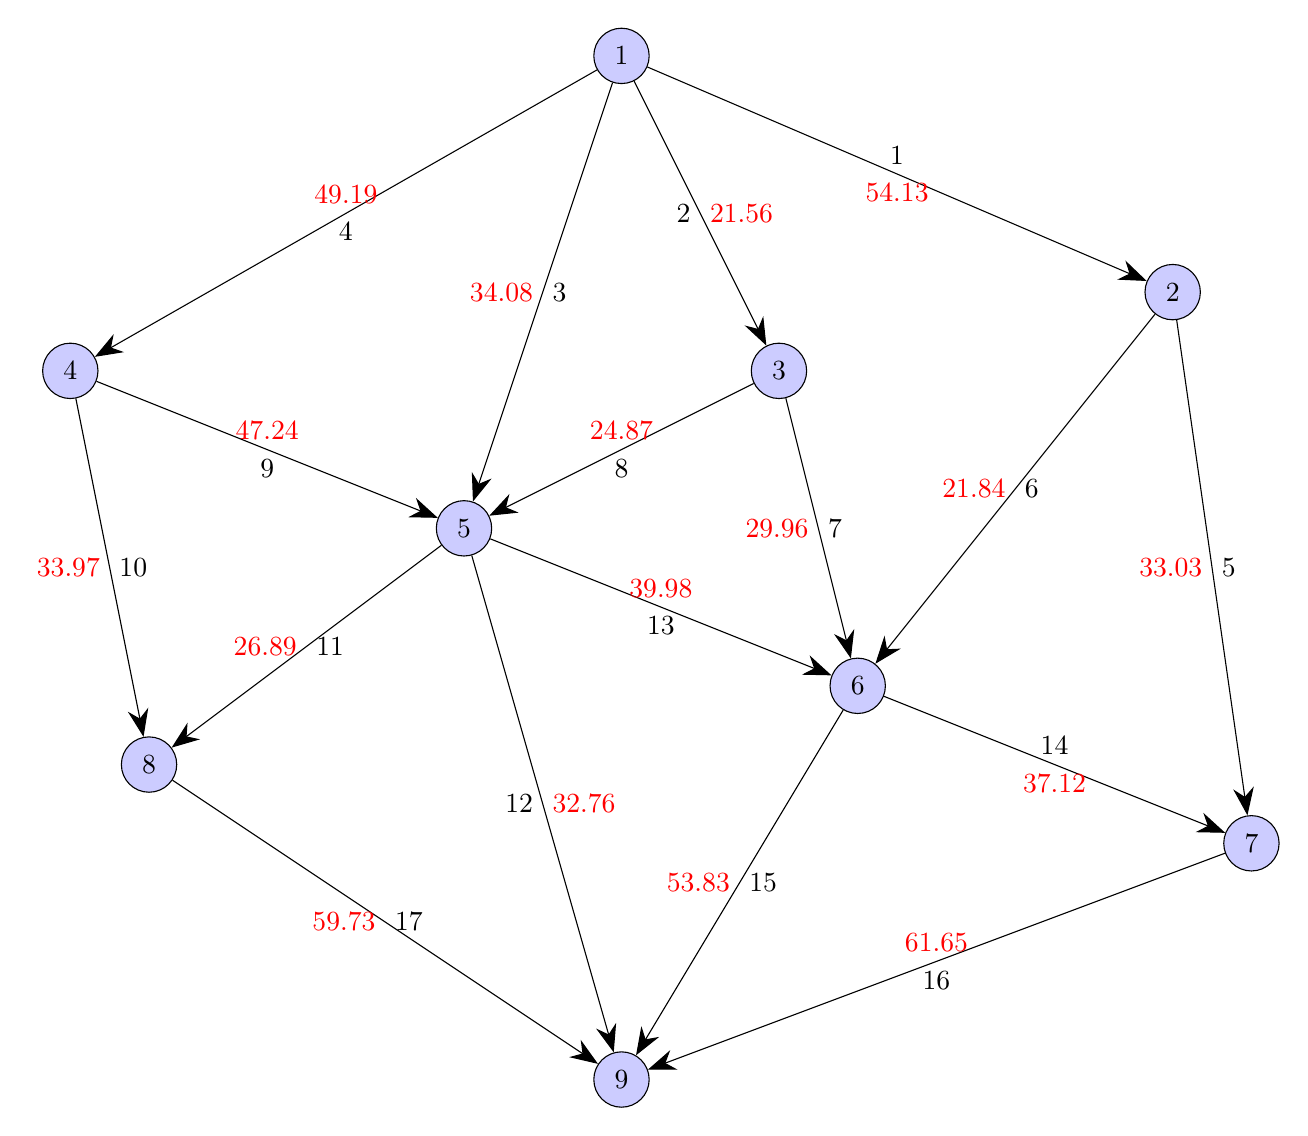
\begin{tikzpicture}[
        xshift=-2cm,  % Shifts the entire figure 2cm to the left
        > = {Stealth[length=10pt]},
        vertex/.style = {circle, draw, fill=blue!20, minimum size=20pt},
        every edge/.style = {draw, ->, thick}
    ]
        % Nodes with increased spacing
        \node[vertex] (v1) at (0,10) {1};
        \node[vertex] (v2) at (7,7) {2};
        \node[vertex] (v3) at (2,6) {3};
        \node[vertex] (v4) at (-7,6) {4};
        \node[vertex] (v5) at (-2,4) {5};
        \node[vertex] (v6) at (3,2) {6};
        \node[vertex] (v7) at (8,0) {7};
        \node[vertex] (v8) at (-6,1) {8};
        \node[vertex] (v9) at (0,-3) {9};
        
        % Edges with centered labels on opposite sides
        \draw[->] (v1) -- (v2) node[midway, above] {1} node[midway, below, red] {54.13};
        \draw[->] (v1) -- (v3) node[midway, left] {2} node[midway, right, red] {21.56};
        \draw[->] (v1) -- (v5) node[midway, right] {3} node[midway, left, red] {34.08};
        \draw[->] (v1) -- (v4) node[midway, below] {4} node[midway, above, red] {49.19};
        \draw[->] (v2) -- (v7) node[midway, right] {5} node[midway, left, red] {33.03};
        \draw[->] (v2) -- (v6) node[midway, right] {6} node[midway, left, red] {21.84};
        \draw[->] (v3) -- (v6) node[midway, right] {7} node[midway, left, red] {29.96};
        \draw[->] (v3) -- (v5) node[midway, below] {8} node[midway, above, red] {24.87};
        \draw[->] (v4) -- (v5) node[midway, below] {9} node[midway, above, red] {47.24};
        \draw[->] (v4) -- (v8) node[midway, right] {10} node[midway, left, red] {33.97};
        \draw[->] (v5) -- (v8) node[midway, right] {11} node[midway, left, red] {26.89};
        \draw[->] (v5) -- (v9) node[midway, left] {12} node[midway, right, red] {32.76};
        \draw[->] (v5) -- (v6) node[midway, below] {13} node[midway, above, red] {39.98};
        \draw[->] (v6) -- (v7) node[midway, above] {14} node[midway, below, red] {37.12};
        \draw[->] (v6) -- (v9) node[midway, right] {15} node[midway, left, red] {53.83};
        \draw[->] (v7) -- (v9) node[midway, below] {16} node[midway, above, red] {61.65};
        \draw[->] (v8) -- (v9) node[midway, right] {17} node[midway, left, red] {59.73};
    \end{tikzpicture}
    \caption{Οδικό δίκτυο}
    \label{fig:traffic_network}
\end{figure}


\end{document}
